\chapter{Conventional Chess Engines}
\label{ch:chess}

State of the art chess computers search into a tree which is branched by the possible moves the players can make. The chosen move is then the move where the most plausible leaf in the tree yields the highest evaluation. Most engines choose to set up this evaluation heuristically, using expert knowledge. Tree search is computationally speaking a very complex operation, which is why branches are pruned as much as possible and heuristics are kept simple to provide fast evaluations. Generally speaking, due to the very time consuming calculations, code is optimized intensively. These optimizations happen in software as well in hardware. To gain computer power, the engines take up most of the CPUs when possible to branch through the search tree, as these operations are highly parallelizable. \\ 
In this chapter, we will look at the principal techniques used in current chess engines. These methods are typically optimized as much as possible to reduce computational overhead. This chapter is divided into four sections, each one describing an important aspect about the determination of the value function of the current board position. This value function is the mapping of a chess board to a score to indicate which side has the best chances. These methods can give an insight in how to improve Deep RL algorithms with respect to chess.\\
First, we will look at how the size of the search tree of possible future moves is reduced in section \ref{sec:search}. Next we consider how to evaluate a board position in section \ref{sec:evaluation}, after which we conclude the chapter by looking into how we can use data intensive knowledge to improve play in section \ref{sec:databases}.

\section{Search}
\label{sec:search}
Due to the tactical nature of chess (i.e. every slightest modification in board configuration can drastically change the evaluation), it seems to be nearly impossible to find an algorithm generating the best move in a blink of an eye. This is why some lookahead is needed to evaluate positions reliably. The search to the best move is done by branching through a tree structure where edges represent moves, and the nodes connected by the edges the positions before and after the move. An example of a search tree is depicted in \ref{fig:searchtree}. \\
One problem is that the search tree grows exponentially for every move made. Suppose we want to look at a depth $d$ (the lateral length of the tree, in this context the maximal number of moves thought ahead) and we can make on average the branching factor $b$ moves every ply, the size of the search tree is $b^{d}$. As chess' branching factor is around 35 \cite{levin14}, the depth is limited very rapidly. At the same time, the deeper an engine can look ahead, the stronger it plays. This is why researchers try to reduce as many branches in the search tree as possible.

%\begin{figure}
%\centering
%\begin{tikzpicture}
%\node[] (root) at (0,0) {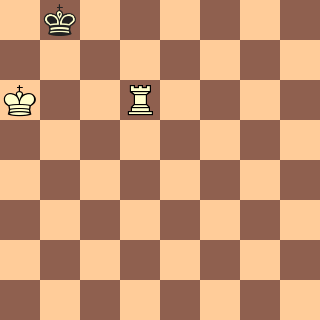
\includegraphics[width=0.1\textwidth]{fig/search/3}};
%%\draw (-)
%
%\node[] at (-1.5,-3) {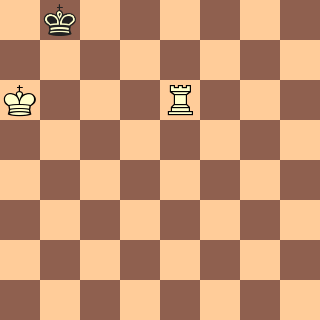
\includegraphics[width=0.1\textwidth]{fig/search/5}};
%\node[] at (-4.5,-3) {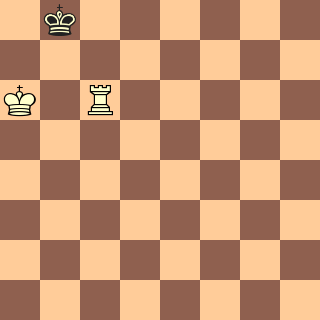
\includegraphics[width=0.1\textwidth]{fig/search/2}};
%\node[] at (4.5,-3) {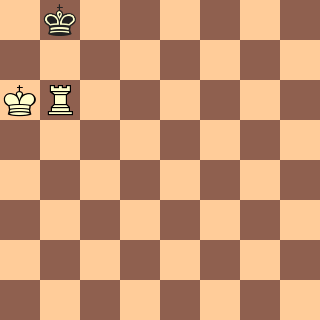
\includegraphics[width=0.1\textwidth]{fig/search/1}};
%\node at (1.5,-3) {$\cdots$};
%
%\node[] at (-4.5,-6) {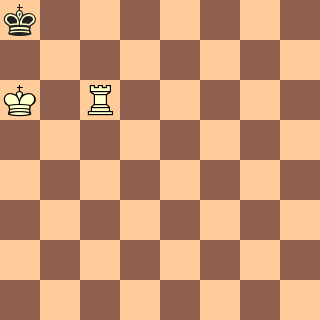
\includegraphics[width=0.1\textwidth]{fig/search/4}};
%\node[] at (2.2,-6) {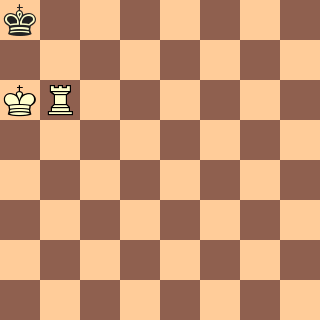
\includegraphics[width=0.1\textwidth]{fig/search/8}};
%\node[] at (6.8,-6) {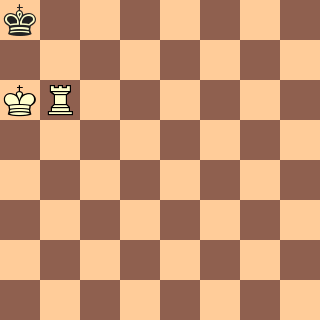
\includegraphics[width=0.1\textwidth]{fig/search/8}};
%
%\node[] at (-4.5,-9) {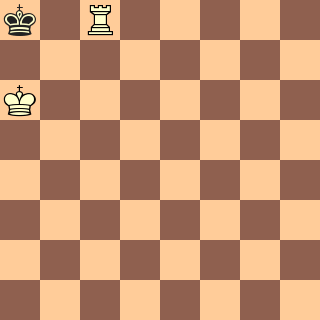
\includegraphics[width=0.1\textwidth]{fig/search/6}};
%\end{tikzpicture}
%\end{figure}

\begin{figure}
\centering
\begin{tikzpicture}[
%level 1/.style={sibling distance=30mm,level distance=3cm},level 2/.style={sibling distance=10mm},level 3/.style={sibling distance=10mm},first/.style={level distance=3cm},
%  second/.style={level distance=3cm,sibling distance=30mm},
%  third/.style={level distance=3cm,sibling distance=30mm},
%  rect/.style={rectangle,minimum size=0.15\textwidth,anchor=south}
	level distance=30mm,
	sibling distance=30mm
  ]
  \tikzstyle{every node}=[rectangle,minimum size=0.15\textwidth]
  
  \node[] {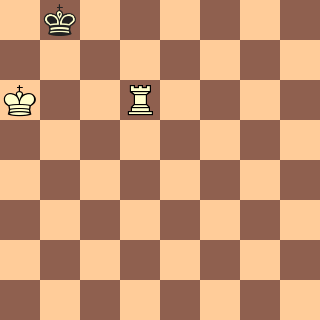
\includegraphics[width=0.15\textwidth]{fig/search/3}} [edge from parent fork down]
  	child{ node[] {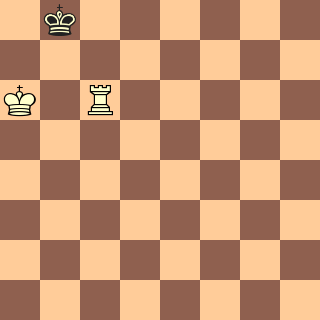
\includegraphics[width=0.15\textwidth]{fig/search/2}}
    		child{node[] {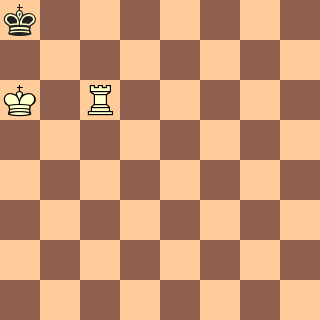
\includegraphics[width=0.15\textwidth]{fig/search/4}}
    			child{node {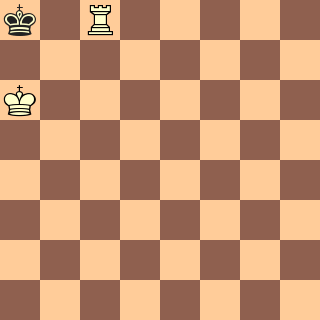
\includegraphics[width=0.15\textwidth]{fig/search/6}}}
    			child{node {$\cdots$}}
    			}
    		}
  	child{ node[] {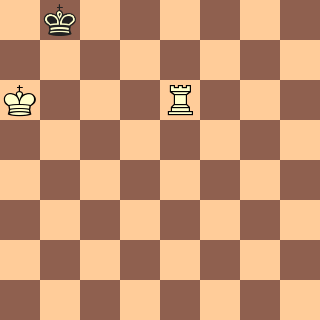
\includegraphics[width=0.15\textwidth]{fig/search/5}}
  		child{node {$\cdots$}}
  		}
  	child{ node[] {$\cdots$}}
  	child{ node[] {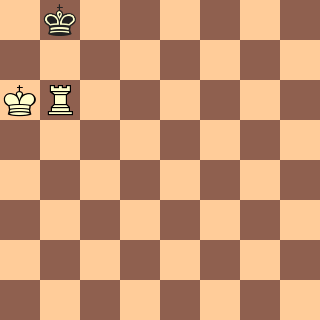
\includegraphics[width=0.15\textwidth]{fig/search/1}}
  		child{node[] {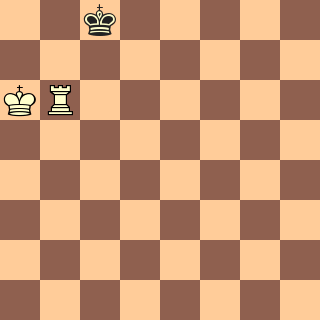
\includegraphics[width=0.15\textwidth]{fig/search/7}}}
  		child{node[] {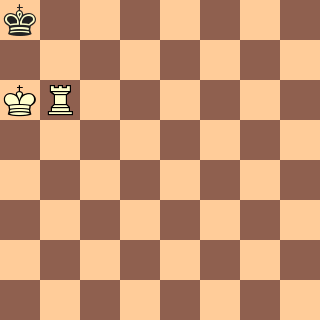
\includegraphics[width=0.15\textwidth]{fig/search/8}}}
  		child{node[] {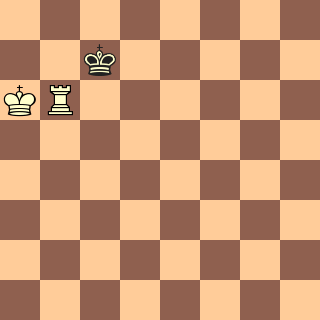
\includegraphics[width=0.15\textwidth]{fig/search/9}}}
  		};

\end{tikzpicture}
\caption[Search tree]{An illustration of a search tree up to $d=3$.}
\label{fig:searchtree}
\end{figure}

\subsection{Minimax}
\label{subsec:minimax}
Minimax is the algorithm describing how to evaluate the root position given the static evaluations of the leaf positions in games. Basically, when we look deeper into the tree, we have to alternately choose between the score of whites and blacks best move. In game theory terminology white and black are called the max-player and min-player, respectively. As the name suggests, the max-player tries to maximize the score while the min-player tries to minimize it. Due to the simplicity of zero-sum games like chess (they are symmetrical, both players try to achieve exactly the same goal, namely checkmating the opponent), the evaluation of a position is equivalent to the negation of the evaluation from the opponent's viewpoint:

\begin{equation}
V^{(w)}(s)\equiv -V^{(b)}(s)
\label{eq:zerosum}
\end{equation}

with $V^{(w)}(s)$ and $V^{(b)}(s)$ the value functions from white and blacks point of view respectively. Value functions indicate the expected outcome of position (an estimated or exact score appropriate to the position).
If one side is winning, the other one is losing. This simplification of minimax with the zero-sum property (also called negamax in literature) is listed as pseudo code in algorithm \ref{al:minimax}.

\begin{algorithm}
  \caption{Minimax}
  \label{al:minimax}
  \begin{algorithmic}
  \REQUIRE board, depth
  \ENSURE  max \\
  \COMMENT{max-player should call \textit{Minimax}(board,depth)} \\
  \COMMENT{first call min-player should be -\textit{Minimax}(board,depth)}
  \IF {depth $\leftarrow 0$}
  \RETURN \textit{Evaluation}(board) 
  \COMMENT{static evaluation of a leaf node}
  \ENDIF

  \STATE max $\leftarrow -\inf$ 
  \FOR{move \textbf{in} \textit{LegalMoves}(board)}
  \STATE newboard $\leftarrow doMove$(board, move)
  \STATE score $\leftarrow -Minimax$(newboard, depth - 1)
  \IF {score $>$ max}
  \STATE max $\leftarrow$ score
  \ENDIF
  \ENDFOR
  \RETURN max
  \end{algorithmic}
\end{algorithm}


\subsection{$\alpha \beta$-pruning}
\label{subsec:alphabeta}
Minimax requires traversing the entire search tree, which is not at all feasible as explained before due to the exponential growth of the search tree. Luckily, an improvement can be made to minimax which allows to safely prune certain subtrees. This improvement is called $\alpha \beta$-pruning, and was already proposed in 1955 \cite{mccarthy55}. The number of nodes to be evaluated is reduced by not traversing nodes further in a branch-and-bound manner when a refutation has been found. In the (recursive) algorithm, two values are stored: $\alpha$ and $\beta$. $\alpha$ represents the minimal score for the max-player in a variation, while $\beta$ represents the maximal score for the min-player. In other words, they are the provisional worst case scenario evaluations for both parties. Based on $\alpha$ and $\beta$, variations can be cut off if proven to involve inferior game play by one of the players. A formal algorithm for games with the zero-sum property is provided in algorithm \ref{al:alphabeta}. Completely worked out examples enhance the understanding significantly, therefore we encourage the reader to look at the cited website \cite{abpractice}. \\
In the worst case, we always evaluate bad leafs and end up with the same complexity of minimax, $O(b^d)$. In the best case scenario, edges corresponding with good moves are traversed first, resulting in hard to beat $\alpha$ and $\beta$ values. By always choosing to branch through the best moves in the search tree we achieve the square root of the original time complexity of minimax $O(b^{\frac{d}{2}})$ \cite{stuart2003}. From this reasoning, it follows that the move ordering of branching is very important, as we could potentially gain twice the depth in our search in the same timespan (see table \ref{tab:alphabeta} for a comparison). Heuristics as well as machine learning techniques like \acrlong{nn}s can be used to determine the move order of the search \cite{hashmoveorder05,nnmovemap02}.

\begin{algorithm}
\caption{$\alpha \beta$Minimax}
\label{al:alphabeta}
\begin{algorithmic}[]
\REQUIRE board, depth, $\alpha$, $\beta$
\ENSURE $\alpha$\\
\COMMENT{max-player should call \textit{Minimax}(board,depthLeft,$-\infty$,$\infty$)} \\
\COMMENT{min-player should call -\textit{Minimax}(board,depthLeft,$-\infty$,$\infty$)}
\IF {depthLeft $\leftarrow 0$}
\RETURN \textit{Evaluation}(board) 
\COMMENT{static evaluation of a leaf node}
\ENDIF
\FOR{move \textbf{in} \textit{LegalMoves}(board)}
\STATE newboard $\leftarrow doMove$(board, move)
\STATE score $\leftarrow -\alpha \beta Minimax$(newboard, depthLeft - 1,$-\beta$,$-\alpha$)
\COMMENT{Exchanging because of zero-sum property}
\IF{score $\geq \beta$}
\RETURN $\beta$
\COMMENT{$\beta$-cutoff}
\ENDIF
\IF{score $> \alpha$}
\STATE{$\alpha \leftarrow$ score}
\COMMENT{$\alpha$ is the max from \textit{Minimax (Algorithm \ref{al:minimax})}}
\ENDIF
\ENDFOR
\RETURN $\alpha$
\end{algorithmic}
\end{algorithm}

\begin{table}[]
\centering
\caption[Comparison $\alpha\beta$-pruning and regular minimax]{The exact number of explored nodes in the best case scenario is $b^{\lceil \frac{d}{2} \rceil}+b^{\lfloor \frac{d}{2} \rfloor}-1 $ \cite{edw61}, while it is $b^{d}$ in regular minimax, which is the worst case for $\alpha \beta$-pruning.}
\label{tab:alphabeta}
\begin{tabular}{rrr}
\toprule
\textbf{depth} & \textbf{worst case} & \textbf{best case} \\
\midrule
0              & $1 \cdot 10^0$                   & $1\cdot 10^0$                  \\
1              & $3.5\cdot 10^1$                & $3.5\cdot 10^1$                 \\
2              & $1.225\cdot 10^3$                & $6.9\cdot 10^1$                 \\
3              & $4.287 \cdot 10^4$  			& $1.259\cdot 10^3$               \\
4              & $1.500\cdot 10^6$             & $2.449\cdot 10^3$               \\
5              & $5.252\cdot 10^7$            & $4.409\cdot 10^4$              \\
6              & $1.838\cdot 10^9$          & $8.574\cdot 10^4$              \\
7              & $6.433\cdot 10^{10}$         & $1.543\cdot 10^6$            \\
8              & $2.251\cdot 10^{12}$       & $3.001\cdot 10^6$            \\
9              & $7.881\cdot 10^{13}$      & $5.402\cdot 10^7$           \\
10             & $2.758\cdot 10^{15}$    & $1.050\cdot 10^8$          \\
\bottomrule
\end{tabular}
\end{table}

\subsection{Principal Variation Search}
\label{subsec:pvs}
\glspl{pvs} (which in literature is often put equal to the almost identical \textit{negascout} algorithm) is a further improvement to the $\alpha \beta$-pruning minimax algorithm which in general leads to a save in computation time when the move ordering is done right. \\ 
The idea is the following: we base our calculations on the principal variation, which is the path in the tree corresponding to the intuitively best move (this could be calculated for example with shallow searches of limited depth). The first node typically traversed is part of the principal variation, after which we continue with regular $\alpha \beta$-pruning. For all the other moves, we set up a small window based (i.e. we suppose $\beta$ to be close to $\alpha$) on the $\alpha$-value found in the principal variation. The immediate consequence is a growing number of $\beta$-cutoffs. If we were to find a variation leading to a score in the window, we know our initial assumption was wrong, and we have to search through the same node once more with general $\alpha \beta$-pruning. This is why the move ordering is crucial for this to work. See algorithm \ref{al:pvs} for pseudo code.\\
\gls{pvs} and negascout yield the same result as $\alpha \beta$-pruning \cite{reine89}. The algorithm is heavily based on the original \textit{Scout} algorithm, which was the first algorithm to outperform $\alpha \beta$-pruning \cite{pearl80}. \\

Another minimax search algorithm has been implemented, proven to outperform \gls{pvs} and negascout in practice, namely \textit{MTD(f)} \cite{plaat96}. The window calls from \gls{pvs} only return a bound on the minimax value. In contrast, MTD(f) calls a full $\alpha \beta$-search a number of times, converging towards the exact value. Overhead of searching through the same nodes is covered by transition tables in memory.

\begin{algorithm}
\caption{PVS}
\label{al:pvs}
\begin{algorithmic}[]
\REQUIRE board, depth, $\alpha$, $\beta$
\ENSURE max \\
\COMMENT{max-player should call \textit{PVS}(board,depth,$-\infty$,$\infty$)} \\
\COMMENT{min-player should call -\textit{PVS}(board,depth,$-\infty$,$\infty$)}
\IF {depth $\leftarrow 0$}
\RETURN \textit{Evaluation}(board) 
\ENDIF \\
\COMMENT{First, calculate score of principal variation with full $\alpha \beta$-search}
\STATE pv $\leftarrow$ \textit{PV}(board)
\STATE newboard $\leftarrow doMove$(board, pv)
\STATE $\alpha \leftarrow$ -\textit{PVS}(newboard,depth$-1$,$-\beta$,$-\alpha$) \\
\COMMENT{Look at other moves in a reduced window $[ \alpha,\alpha +1]$ \cite{fishburn84}}
\FOR{move \textbf{in} \textit{LegalMoves}(board) \textbf{and} move $\neq$ pv}
\STATE newboard $\leftarrow doMove$(board, move)
\STATE score $\leftarrow -PVS$(newboard, depth - 1,$-\alpha-1$,$-\alpha$)
\IF{$\alpha < $score$ < \beta$}
\STATE score $\leftarrow -PVS$(newboard, depth - 1,$\beta$,$-\alpha$)
\COMMENT{Wrong guess of pv, full research}
\ENDIF
\IF{score $\geq \beta$}
\RETURN $\beta$
\COMMENT{$\beta$-cutoff}
\ENDIF
\IF{score $> \alpha$}
\STATE{$\alpha \leftarrow$ score}
\ENDIF
\ENDFOR
\RETURN $\alpha$
\end{algorithmic}
\end{algorithm}

\subsection{Quiescence Search}
\label{subsec:qs}
A remaining problem after the already presented search algorithms is the fixed depth. This can cause the horizon effect, the evaluation at the leaf node can be suboptimal due to the possible presence of tactical moves completely changing the static evaluation. An example of how problematic this can be is shown in figure \ref{fig:qs}. \\
Typical tactical moves that are considered are piece captures and checks. The search goes on until the node seems 'quiet' enough, or by finding a new lower bound to the minimax score with a static evaluation \cite{beal90}. This enhancement is based on the null move observation, which expresses that it is (almost \footnote{In rare cases, no good moves are available, and a player is forced to weaken its position. These positions are called zugzwang positions}) always better for the side to move to play than to do nothing.

\begin{figure}
    \centering
    \begin{subfigure}[b]{0.3\textwidth}
        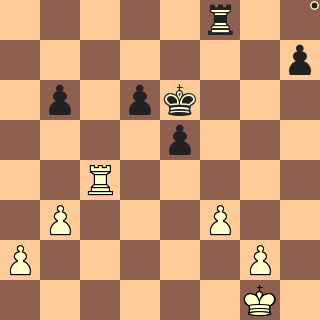
\includegraphics[width=\textwidth]{fig/diagram_qs_1}
        \caption{Black to move}
        \label{fig:qs1}
    \end{subfigure}
    ~ %add desired spacing between images, e. g. ~, \quad, \qquad, \hfill etc. 
      %(or a blank line to force the subfigure onto a new line)
    \begin{subfigure}[b]{0.3\textwidth}
        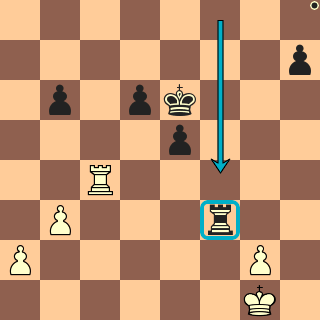
\includegraphics[width=\textwidth]{fig/diagram_qs_2}
        \caption{White to move}
        \label{fig:qs2}
    \end{subfigure}
    ~ %add desired spacing between images, e. g. ~, \quad, \qquad, \hfill etc. 
    %(or a blank line to force the subfigure onto a new line)
    \begin{subfigure}[b]{0.3\textwidth}
        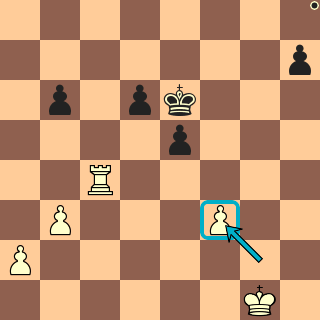
\includegraphics[width=\textwidth]{fig/diagram_qs_3}
        \caption{Black to move}
        \label{fig:qs3}
    \end{subfigure}
    \caption[Importance quiescence search]{Suppose the remaining depth after figure \ref{fig:qs2} is 0, then a static evaluation of the position is required. Without any \gls{qs}, a typical engine would first of all count all the pieces on the board and note that black is a pawn up, hence yield an evaluation in favor of black. This is utterly wrong, as white is winning in this position, due to the tactical change at the next move gxf3. Now White is a Rook up in exchange of a pawn. The figure \ref{fig:qs3} shows the resulting position after the exchange. There are no remaining tactical threats in this position, hence this is a quiet position. The engine should have computed this as well to provide a reliable minimax evaluation.}
    \label{fig:qs}
\end{figure}

\subsection{Other Search Improvements}
\label{subsec:others}
In this subsection, we briefly discuss other possible (some of them obligatory) enhancements to regular $\alpha \beta$-search. \\

While traversing through the search tree, stakes are high chess engines encounter the same states again and again (but achieved through different paths). This is why a transposition table is stored in memory, which is essentially a large hash table storing information about all encountered positions \cite{kishimoto02}. Typical characteristics that are stored in an entry are
\begin{itemize}
\item best move
\item highest calculated depth
\item score
\end{itemize}

Another almost obligatory enhancement on the basic methodology is iterative deepening. Because of the exponential complexity and uncertainty about the duration of searching (e.g. in \gls{qs}), time management is required. Some time is allocated for the search of a best move, and systematically the calculations go deeper and deeper. In case of time running out, the engine can still fall back to the best move according to current calculations, this as opposed to to depth first searches. Usually, the depth first algorithms like $\alpha \beta$-pruning (as we have seen in previous sections) are fit into a best first framework \cite{korf85,reine94}. \\

In section \ref{subsec:pvs} we saw that a more narrow window was used in \gls{pvs} as a way to achieve more cutoffs in $\alpha \beta$-search. Aspiration windows use the same idea, they make a guess about the size of the window. If the true score appears to be outside this window, a costly re-search has to be made. To mitigate this downside, some programs change the window size according to fails. For example, if the windows fail by estimating $\beta$ too low, an engine will typically increase the upper bound.

\section{Evaluation}
\label{sec:evaluation}
How do we give a static evaluation to a leaf node in the search tree? The exact value is unknown unless we have arrived (close to) a terminal state, so we have to make an approximation. In conventional chess engines heuristics are applied to perform these approximations. This comes at the cost of being biased by human expert knowledge, which is difficult to prove to be entirely correct. Examples can be found where the computer does not seem to find the best move or interpret the position correctly. \\

We are not going to discuss this in great detail, but generally a big amount of features is extracted from the position, and every feature gets a weight. Engines use these weights to describe the dynamics between these features and their relative importance. Most evaluation functions in existing chess engines use a linear value function
\begin{equation}
V({s})=\sum_{f \in \mathcal{F}} w_i f 
\end{equation}
where \textit{s} denotes the state of the board (the chess position). The weights represent the importance of every feature to the global evaluation, e.g. the value of the pieces on the board will have a larger weight than structural characteristics. Nonlinear evaluation functions can be used as well, but are due to speed less common at the moment of writing. Typical features considered are among other more complex ones:
\begin{itemize}
\item material
\item pawn structure
\item piece mobility
\item connectivity
\item king safety
\end{itemize}
The weights of features also depend on the game phase. Most evaluation functions make a distinction between the opening, middlegame and endgame. These are all hand crafted characteristics about the chess game humans discovered by themselves, and each player from beginner to expert tries to learn the dynamics between the importance of these features through game play.

\subsubsection*{Tuning}
Tuning is the subject about how to automatically adjust the weight to achieve the highest possible playing strength. This can be done with supervised learning (section \ref{sec:ml}), \acrlong{rl} (section \ref{sec:rl}), genetic algorithms as used in \textit{Falcon} \cite{tabib09}, but also with other less mathematically sound mechanisms. \textit{Stockfish} for example assures that the weights of the most important features reach their optimal values rapidly based on game play between engines differentiated through the variables, which accompanies a gain of strength. One issue is that after the optimization of the important variables, the less significant variables take a random walk and playing strength may decrease \cite{joona11}.\\

To perform reliable automated tuning, a change in playing strength should somehow be measured. This is faced with some difficulties, as chess is a game containing a lot of diversity. How does one generate an adequate set of test positions? How are we certain all aspects of the game have been covered? The solution is to play as many randomized (preferably realistic in practice) positions between engine opponents. The standard way to do this is to play many games with a small time control, where games can end prematurely. Strength of an engine (or chess player in general) is calculated with the ELO rating system (section \ref{sec:elo}).
%PUT FIGURE IN%

\section{Databases}
\label{sec:databases}

\subsection{Opening Books}
\label{subsec:opening_books}
Probably the most complex phase of a chess game is the opening. Strategically and tactically it is a very challenging part of the game, and grandmasters often lose games due to slight inaccuracies in opening play. This is why grandmasters prepare their games by revising their opening play depending on the typical opening choices of their opponents. If the chess player is well prepared, he may automate the first moves and save a considerable amount of time, which may come out beneficially at time control. \\
An identical argument can be made in favor for an engine storing an opening book, which is basically a tree of chess moves starting from the initial position. All lines stored in an opening book are expert knowledge, chess theory evolved throughout history. \\

Chess theory may contain bad lines, this is why book learning is implemented in \textit{Crafty} \cite{hyatt1999,Kloetzer2011}. When many games through the same leaf node of the opening tree are lost, this node is removed. Hence, this is a trial and error mechanism. This bad book move signaling can remove bad lines.

\subsection{Endgame Tablebases}
\label{subsec:tablebases}
Since August 2012, chess has been solved completely up to seven pieces (kings included) by a supercomputer at \textit{Moscow State University}. The idea of a tablebase is to store a database containing the \gls{dtm} (number of moves up until checkmate) from all winning positions. All absent positions in the database are theoretical draws. By using a tablebase, we only have to maximize the \gls{dtm} of all possible moves to achieve optimal play. Tablebases can be uploaded into engines, which will look up the position into the database and play the best move. Although they do not contain all positions up until seven pieces (this takes 130 000 GB on a hard drive), it greatly simplifies computations for plenty endgame scenarios \cite{lomonosov12}.\\

Tablebases have been generated with retrograde analysis, from all possible checkmate positions calculations worked backwards. This technique has unveiled winning sequences which are beyond human comprehension. The coming of tablebases has put the 50-move rule under pressure, although most 50+ winning sequences are a set of seemingly random piece dancing. An example has been provided in Figure \ref{fig:mate549}. \\

\begin{figure}
\centering
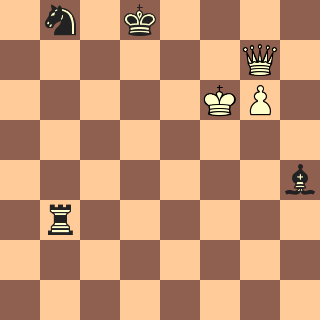
\includegraphics[width=6cm]{fig/mate_in_549}
\caption[Mate in 549]{White to move can mate black in a forced way in an exuberant number of 549 moves. No engine can find the right sequence. This problem is left as an exercise to the reader}
\label{fig:mate549}
\end{figure}

\section{Conclusion}
\label{sec:chessconclusion}

To conclude this chapter, we analyze the characteristics of these approaches. Although chess engines today are much stronger than professional human players (compare the rating of the world champion which is around 2800 with table \ref{tab:engines}), we can never be sure with this approach if the engines are actually making the best decisions. These engines are designed in such a way that they do not play intuitively, but calculate as much variations as possible and base their decision upon that. The choices of variations to look at are based on human expert knowledge, hence the state of the art chess computers have been taught to choose actions in their search tree by human guidelines. \\
These choices have especially their consequences for positional and endgame play, which are far from optimal right now. The static position evaluations have been decided heuristically, which may not have been generalized enough for all chess positions (an example over-coloring this aspect is illustrated in figure \ref{fig:toy}).\\
Due to the tree operations in the search algorithm, there is often overhead by traversing bad lines. A lot of effort has been put in the selection of lines when branching through the tree by introducing heuristics into the move order. If the engines would somehow have better intuition in this idea, the computational effort could decrease.\\
Globally, these methods have already been optimized so much with parallelization and small optimizations, that it may be time to look for different methods to learn more about the beautiful game.

\begin{table}[]
\centering
\caption[Strongest chess engines]{The 12 strongest chess engines, tested by letting them play against each other. These are the playing conditions: Ponder off, General book (up to 12 moves), 3-4-5 piece EGTB
Time control: Equivalent to 40 moves in 40 minutes on Athlon 64 X2 4600+ (2.4 GHz), about 15 minutes on a modern Intel CPU.
Computed on May 27, 2017 with Bayeselo based on 715'938 games \cite{engines}. The strongest FIDE chess rating ever recorded (May 2014) attained by the world champion Magnus Carlsen (at the moment of writing) is included in the ranking for comparison.}
\label{tab:engines}
\begin{tabular}{rrrr}
\toprule
\textbf{Rank} & \textbf{Name} & \textbf{Rating} &\textbf{95\% Confidence} \\
\midrule
1 & Komodo 10.4      & 3392 & $[3372,3412]$ \\
2 & Stockfish 8      & 3390 &  $[3373,3407]$\\
3 & Houdini 5.01     & 3387 & $[3368,3406]$ \\
4 & Deep Shredder 13 & 3288 & $[3268,3308]$ \\
5 & Fire 5           & 3270 & $[3248,3292]$ \\
6 & Fizbo 1.9        & 3249 & $[3225,3273]$ \\
7 & Andscacs 0.89    & 3240 & $[3216,3264]$ \\
8 & Chiron 4         & 3208 & $[3184,3232]$ \\
9 & Gull 3           & 3194 & $[3183,3205]$ \\
10 & Equinox 3.20     & 3186 & $[3174,3198]$ \\
11 & Booot 6.1        & 3178 &  $[3157,3199]$\\
12 & Fritz 15         & 3171 & $[3158,3184]$ \\
&$\cdots$&&\\
58 & Magnus Carlsen & 2882 &\\
\bottomrule
\end{tabular}
\end{table}

\begin{figure}
\centering
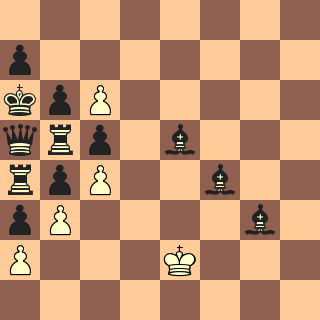
\includegraphics[width=6cm]{fig/diagram_eval}
\caption[Toy example]{A toy example where chess engines fail to indicate the right evaluation. Because the static evaluations are favoring the material value count against the structure in an unbalanced way in this position, the computers indicate black will win almost certainly. In reality, white can actually force this game to be a draw relatively easily \cite{toy}.}
\label{fig:toy}
\end{figure}